\def\QRCODE{TB_IPR_TUT.IMG.integral_geometry_pythonqrcode.png}
\def\QRPAGE{http://www.iptutorials.science/tree/master/TB_IPR/TUT.IMG.integral_geometry/python}
\pcorrectionsection{Python correction}

\subsection{Cell configurations}

The following values are reported:
\begin{eqnarray*}
 f^{intra}=50 \\
 e^{intra}=158 \\
 v^{intra}=107
\end{eqnarray*}

\begin{eqnarray*}
 f^{inter}=4 \\
 e^{inter}=42 \\
 v^{inter}=50
\end{eqnarray*}

Then, it is easy to compute the following values:

\begin{eqnarray*}
A&=&f^{intra}=50\\
P&=&-4f^{intra}+2e^{intra}=116\\
\chi_8&=&v^{intra}-e^{intra}+f^{intra}=-1\\
\chi_4&=&v^{inter}-e^{inter}+f^{inter}=12
\end{eqnarray*}

\subsection{Neighborhood configuration}

The configuration is computed using the convolution function \pinline{scipy.signal.convolve2d}. The histogram of the different configurations is presented in Fig.\ref{fig:integral_geometry:python:histo}.

Be aware that this algorithms works if there is no object pixel touching the borders of the image. The example image is in this case, but you can ensure this property by padding 0 values around the image:
\begin{python}
X = np.pad(I, ((1,1),), mode='constant');
\end{python}

\begin{python}
# Neighborhood configuration
F = np.array([[0, 0, 0], [0, 1, 4], [0, 2, 8]]);
XF = signal.convolve2d(X,F,mode='same');
edges = np.arange(0, 17 ,1);
h,edges = np.histogram(XF[:],bins=edges);
plt.figure()
plt.bar(edges[0:-1], h);
plt.title("Histogram of the different configurations")
plt.show() 
\end{python}

\begin{figure}[htbp]
\centering
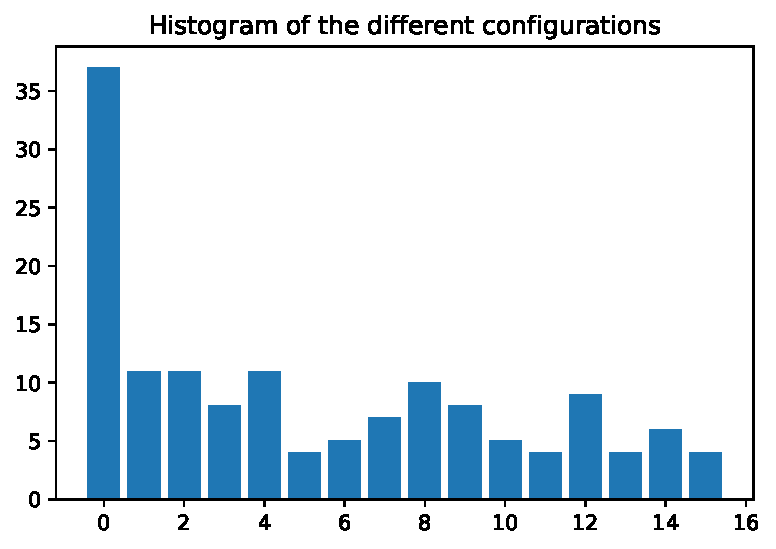
\includegraphics[width=.5\textwidth]{histo.pdf}
\caption{Distribution of the different neighborhood configurations.}
\label{fig:integral_geometry:python:histo}
\end{figure}

The Minkowski functionals are computed using the cells contributions:
\begin{python}
# Computation of the functionals
f_intra = [0,1,0,1,0,1,0,1,0,1,0,1,0,1,0,1];
e_intra = [0,2,1,2,1,2,2,2,0,2,1,2,1,2,2,2];
v_intra = [0,1,1,1,1,1,1,1,1,1,1,1,1,1,1,1];
EulerNb8 = np.sum(h*v_intra - h*e_intra + h*f_intra)
f_inter = [0,0,0,0,0,0,0,0,0,0,0,0,0,0,0,1];
e_inter = [0,0,0,1,0,1,0,2,0,0,0,1,0,1,0,2];
v_inter = [0,1,0,1,0,1,0,1,0,1,0,1,0,1,0,1];
\end{python}

Then, the values are easily verified.
\begin{python}
EulerNb4 = np.sum(h*v_inter - h*e_inter + h*f_inter)
Area = sum(h*f_intra)
Perimeter = sum(-4*h*f_intra + 2*h*e_intra)
print("E_4:{0}, A:{1}, P:{2}".format(EulerNb4, Area, Perimeter));
\end{python}

\begin{sh}
E_4:12, A:50, P:116
\end{sh}


\subsection{Crofton perimeter}
The Crofton perimeter is a good approximation of a perimeter. One should notice that there is no definitive solution to perimeter evaluation. The Crofton perimeter is approximated in 2 or 4 directions, denoted $P_4$ and $P_8$ with a reference to the connectivity.

\begin{python}
# Crofton perimeter
P4 = [0,np.pi/2,0,0,0,np.pi/2,0,0,np.pi/2,np.pi,0,0,np.pi/2,np.pi,0,0];
Perimeter4 = sum(h*P4)
P8 = [0,np.pi/4*(1+1/(np.sqrt(2))),np.pi/(4*np.sqrt(2)),np.pi/(2*np.sqrt(2)),0,np.pi/4*(1+1/(np.sqrt(2))),0,np.pi/(4*np.sqrt(2)),np.pi/4,np.pi/2,np.pi/(4*np.sqrt(2)),np.pi/(4*np.sqrt(2)),np.pi/4,np.pi/2,0,0];
Perimeter8 = sum(h*P8)
\end{python}

\begin{sh}
Perimeter4: 91.10618695410399, Perimeter8: 77.76399477870015
\end{sh}
